\chapter{ミラー計測実験}
\thispagestyle{empty}
\label{chap5}
\graphicspath{{chap5/figure/}}
\minitoc

\newpage
%%%%%%%%%%%%%%%%%%%%%%%%%%%%%%%%%%%%%%%%%%%%%%%%%%%%%%%%%%%%%%%%%%%%%%%%%%%%%


% ================================================== %
% section
% ================================================== %
\section{諸言}
\label{chap5_introduction}

本章では、実際に天文用Wolterミラーを\ref{chap3}章の提案手法による計測実験を行い、その解析を行う。
測定対象となるミラーは、東京大学の三村グループによって2021年1月に作製された天文用Wolterミラーであり、これらの設計パラメータは1章\ref{chap1_wolter_arrangement}に示した通りである。
この3枚のミラーそれぞれについて位相回復計算を行った結果、およびその繰り返し計測精度と回転角度を変えた場合の整合性について述べる。

\clearpage
% ================================================== %
% section
% ================================================== %
\newpage

\section{実験の構成}

実験装置の概要を図\ref{fig:mirror_experiment_schematic}に示す。
まず、レーザーからビームを出力し、これをNDフィルタによって減衰させ、強度を調整する。
次に、レンズを2つ使ってビームを拡大し平行化する。
これを測定対象のWolterミラーに入射し、さらにタイコグラフィのための回転ピンホールを通過させる。
最後に、一番下流にあるCCDカメラで強度分布を撮影する。

\begin{figure}[!ht]
\centering
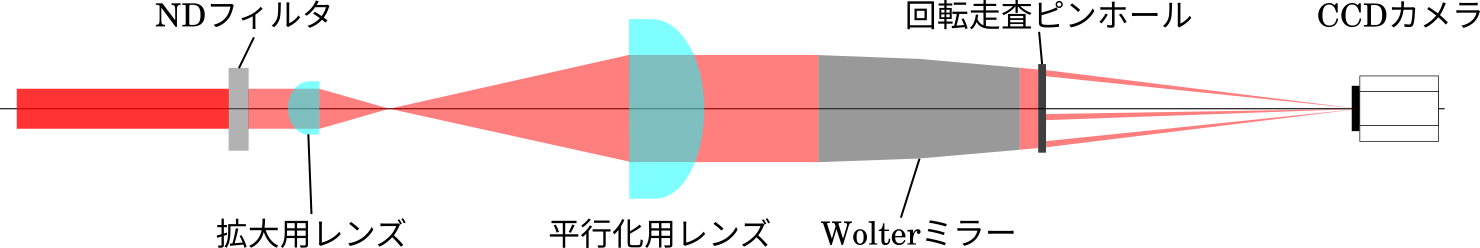
\includegraphics[width=13cm]{mirror_experiment_schematic.png}
\caption{ミラー測定実験系 模式図}
\label{fig:mirror_experiment_schematic}
\end{figure}

これらの光学素子のパラメータを表\ref{tb:mirror_experiment_params}に示す。
なお、NDフィルタは実験によって適宜ピークがダイナミックレンジに収まるように設定されるため、そのパラメータ等を記述しない。

\begin{table}[h]
\begin{center}
  \begin{tabular}{|c|c|} \hline
    パラメータ & 値 \\ \hline
    ビーム波長 & 632.8 nm  \\
    ビームサイズ($\text{TEM}_{00} 1/e^2$点 +3\%) & 0.63 mm  \\
    ビーム発散角度($\text{TEM}_{00}$ +3\%) & 1.3 mrad  \\
    拡大用レンズ焦点距離 & 8.0 mm  \\
    平行化用レンズ焦点距離 & 800.0 mm  \\
    拡大倍率 & 100 倍 \\
    レンズ設計波長 & 541.6 nm \\ \hline
  \end{tabular}
  \caption{Wolterミラー計測実験装置における各素子のパラメータ}
  \label{tb:mirror_experiment_params}
\end{center}
\end{table}

これらを構成した実験装置のCAD図を以下に示す。図\ref{fig:mirror_experiment_asm_cad_side}が横から見た図、図\ref{fig:mirror_experiment_asm_cad_isometric}が俯瞰して見た図である。

\begin{figure}[!ht]
\centering
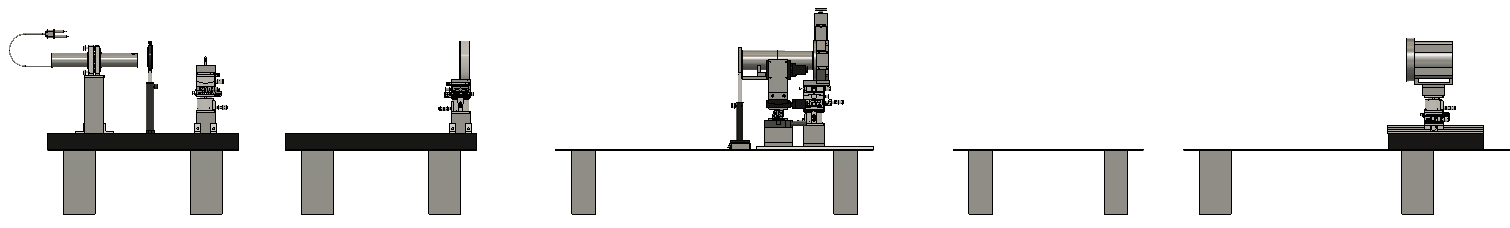
\includegraphics[width=14cm]{asm_total_side.png}
\caption{ミラー測定実験系 側面図}
\label{fig:mirror_experiment_asm_cad_side}
\end{figure}

\begin{figure}[!ht]
\centering
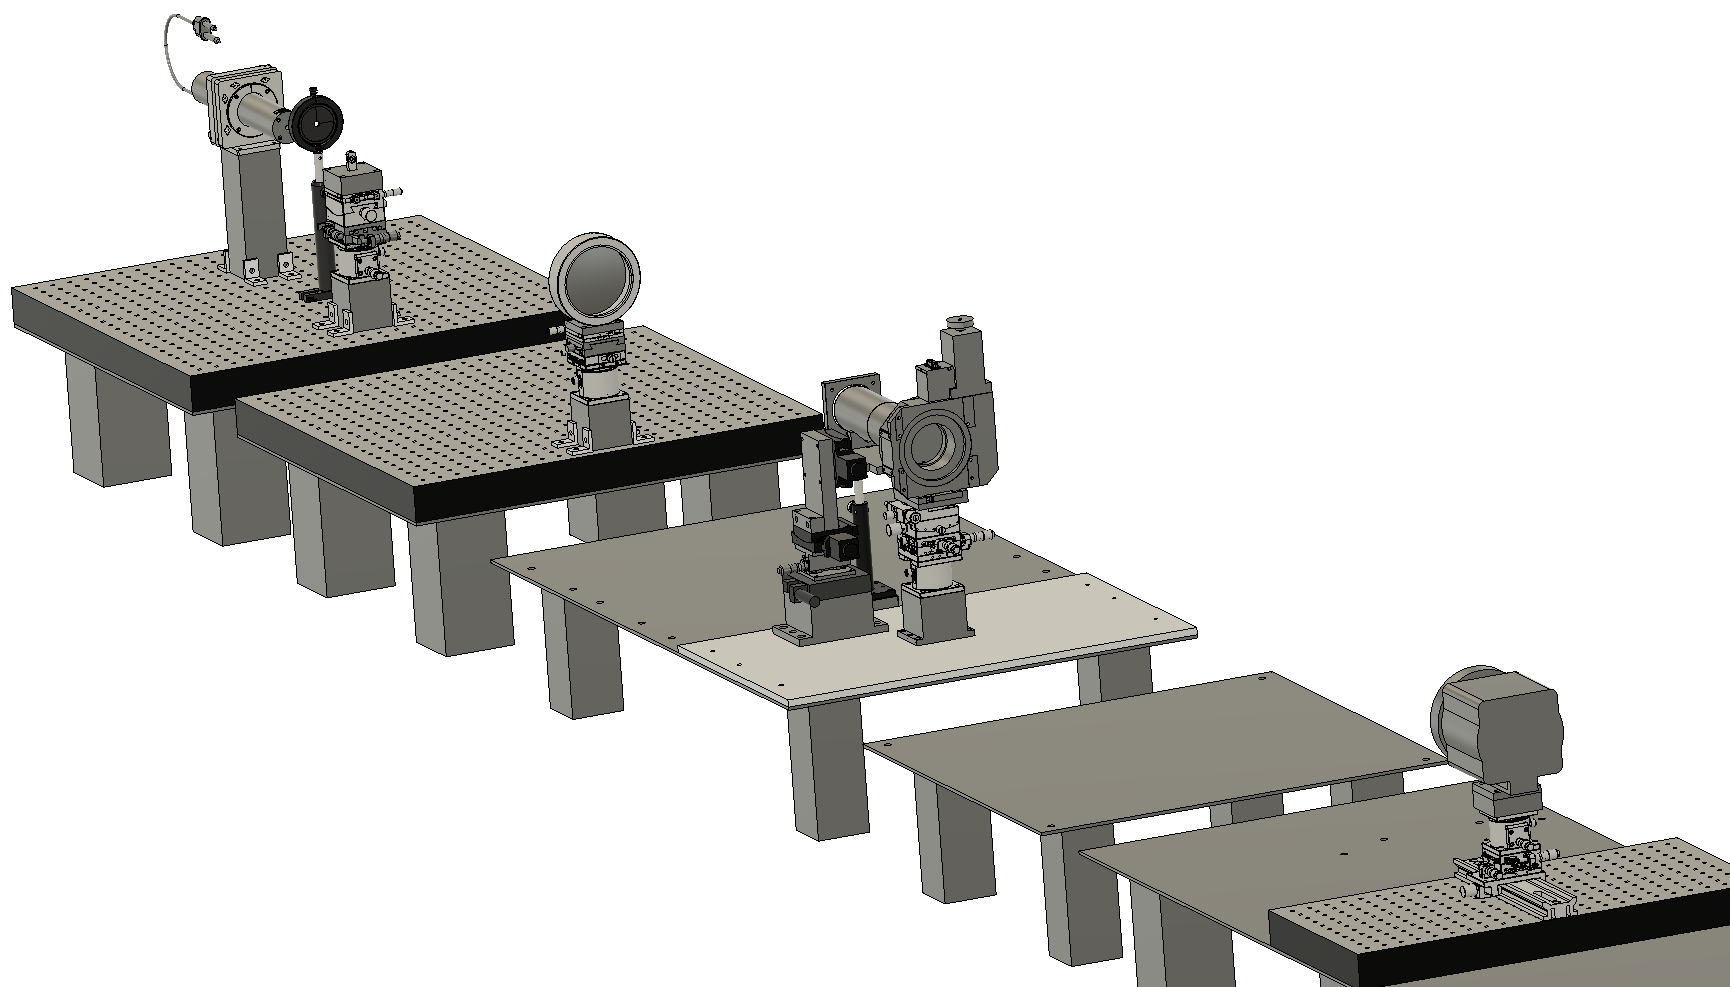
\includegraphics[width=10cm]{asm_total_isometric.png}
\caption{ミラー測定実験系 俯瞰図}
\label{fig:mirror_experiment_asm_cad_isometric}
\end{figure}


\subsection{ミラーの把持}
回転体ミラーの測定実験系を構成する上で、ミラーの把持は一つの問題となる。
板型ミラーの場合であれば、反射面以外の平面部を挟むようにして把持することができる。
一方で円筒型の薄いミラーの場合そのような部分はなく、できるだけ小さな応力で、かつ設置位置に決まった位置に収まるように把持しなければならない。
そこで、仙波らの方法にならい、Bessel点で触れるように下から把持する機構を採用する。\cite{Senba2010}
Bessel点は均等荷重を受ける2点支持された梁の重力によるたわみ量が最小となるような点であり、梁の全長$L$に対して、梁の両端から内側に向かって約$0.2203L$(あるいは中心から$\pm 0.2797 L$)の位置として計算される。
ミラーは光軸上の位置によって半径が異なり厳密には均等荷重ではないが、斜入射が小さくほぼ真円筒とみなせるため、近似的な範囲ではこれで十分であると考えた。
測定対象のミラー全長220 mmに対してBessel点は中心から約$\pm$61.53 mmであり、これを採用した把持機構は図\ref{fig:mirror_holder_jig}のようになった。
ミラーと治具の接触点は赤点で示す通りである。

\begin{figure}[!ht]
\centering
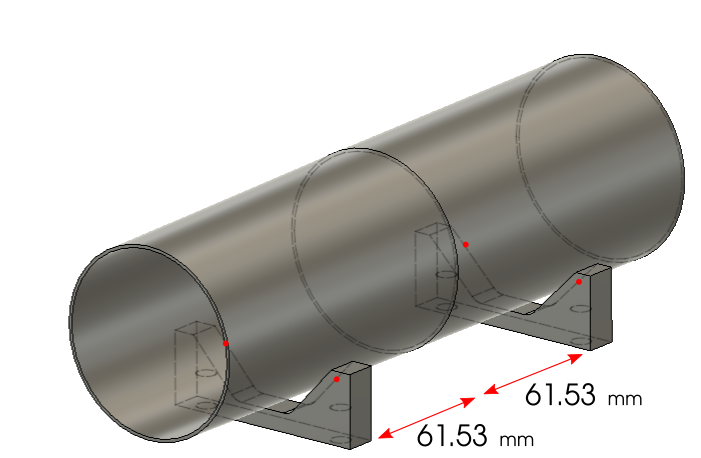
\includegraphics[width=10cm]{mirror_holder_jig.png}
\caption{ミラー把持部の設計図}
\label{fig:mirror_holder_jig}
\end{figure}

また、ミラーを置き直した際に設置位置の繰り返し再現性が高い方が、アラインメントに関して有利である。
光軸方向の距離を合わせるため、ミラー上流端においてミラーの厚み1mmに対してちょうどその半分の位置に当たるような治具を配置し、これに対して押し付けるようにミラーを設置した。
実際に組み立てられた装置は図\ref{fig:photo_mirror_experiment_mirror_and_pinhole}のようになった。

\begin{figure}[!ht]
\centering
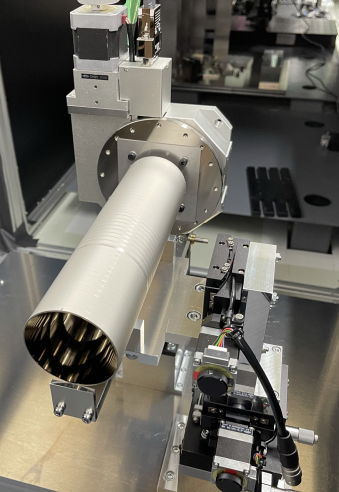
\includegraphics[width=5cm]{photo_mirror_pinhole.png}
\caption{ミラー測定実験系 写真}
\label{fig:photo_mirror_experiment_mirror_and_pinhole}
\end{figure}


\subsection{ピンホールの設計}

ピンホールの設計は図\ref{fig:mirror_pinhole_arrangement}に示す通りである。
断りとして、以下の設計が2つの誤謬を孕んでいることを述べておく。
1つは、ピンホール中心が移動する円の直径はちょうど計測する輪帯状波面のちょうど半分の直径とするのが自然だが、そのような直径を持つ円に対して1つのピンホールが対応する角度を先に決めて、その角度を持つ扇形の弦が直径となるように円を定めている。
もう1つは、シミュレーション上で回復ができると判断した半径2.25 mmの円に対して、直径2.25 mmとしてしまったことである。
これによって、上の計算にはもはや意味を失っている。
ただ、測定対象の輪帯がピンホール通過領域に収まれば問題はなく、直径の決め方は些細な問題である。

\begin{figure}[!ht]
\centering

\subfloat[ピンホールの設計]{
    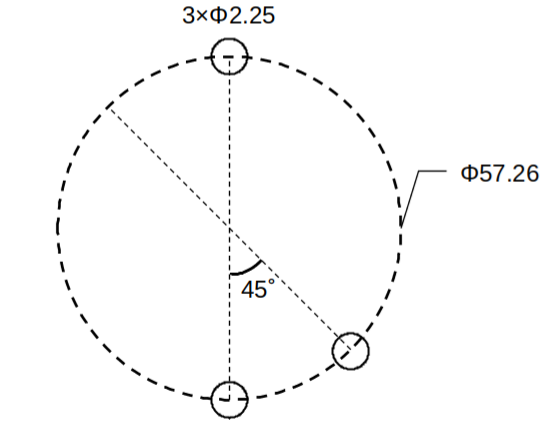
\includegraphics[width=7cm]{pinhole_arrangement.png}
    \label{fig:mirror_pinhole_arrangement}
}
\subfloat[回転半径の決め方]{
    \centering
    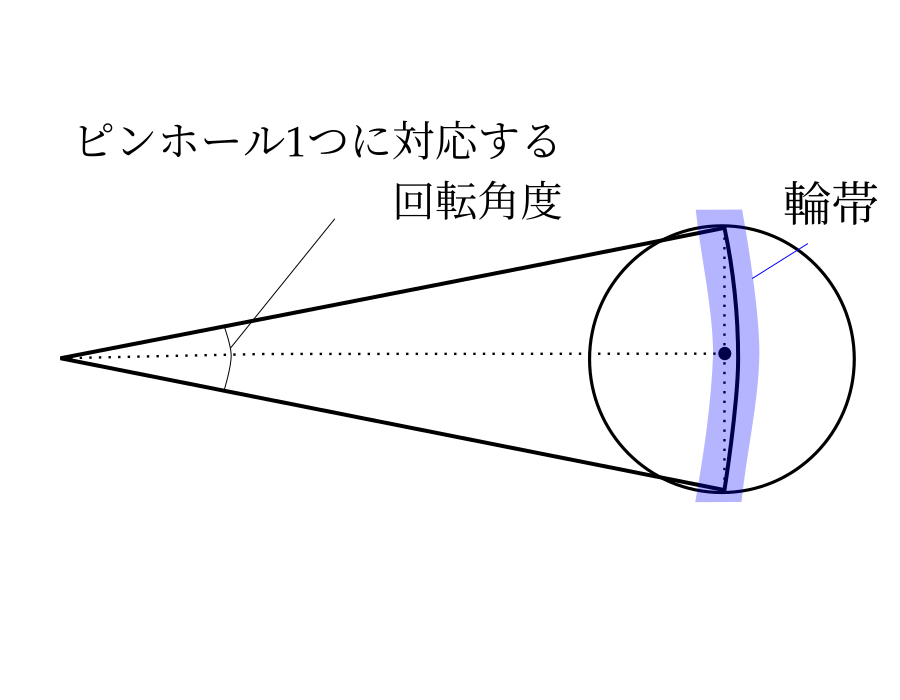
\includegraphics[width=6cm]{pinhole_arrangement_policy.png}
    \label{fig:mirror_pinhole_arrangement_policy}
}
\caption[]{ピンホールの設計}
\label{fig:pinhole_arrangement_pictures}
\end{figure}


\clearpage
% ================================================== %
% section
% ================================================== %
\newpage

\section{計測波面以外の通過光の処理方法に関する検討}
測定対象となっている天文用Wolterミラーは、X線集光用に設計・作製されたものであり、可視光を入射した際にどのような集光波面が生じるかは未検討である。
\ref{chap4}章での提案手法の検討は、あくまで波面計測の対象である輪帯のみが存在する場合について行われたが、実際にミラーを計測する実験においては測定対象以外の光も通過してCCDカメラの方向に進行する。
円形の平行光を入射した際にミラーより下流に通過する光は、図\ref{fig:mirror_beam_path_types}に示す通り3種類存在する。
1つは計測対象の2回反射光、1つは放物面には当たらず双曲面で1回だけ反射された光、1つは直接通過光である。

\begin{figure}[!ht]
\centering
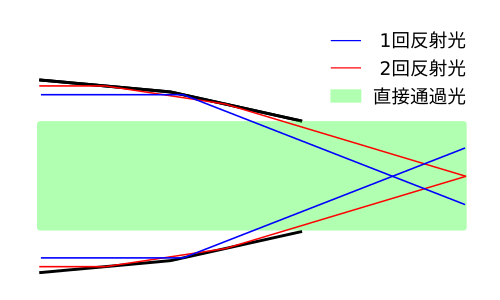
\includegraphics[width=10cm]{reflection_beam_types.png}
\caption{ミラーに入射した光の進路}
\label{fig:mirror_beam_path_types}
\end{figure}

直接通過光は、ピンホールの金属板によって遮蔽されており、またピンホールを通過してもCCDカメラの撮影領域から10 mm以上外れているためこれは計測強度値に影響を及ぼさない。
双曲面による一回反射光は、焦点面において直径約30 mmとなるため、CCDカメラに入射してしまう。
これを取り除く方法は2種類考えられる。
1つは、撮影される強度分布において1回反射光を含まない領域を切り出し、これを回復に用いる方法、もう1つは集光点より上流に存在する1回反射光の集まる位置でこれを遮蔽するという方法である。
前者では切り出しを行ったとしてもその回折光は入射してしまうほか、焦点面サイズを狭めることになるため下流端面の空間分解能が低下してしまう。
後者では集光ビームを遮ることなく遮蔽することはほとんど不可能である上、遮蔽板のエッジで回折した光はまた焦点面の強度分布に影響を及ぼしてしまう。
いずれも大きな問題を抱えているが、本実験では構成が簡単な前者を選択することとする。


\clearpage
% ================================================== %
% section
% ================================================== %
\newpage

\section{撮影条件およびデータの処理}

\subsection{撮影条件}
撮影時の条件を表

\begin{table}[!ht]
\begin{center}
  \begin{tabular}{|c|c|} \hline
    パラメータ & 値 \\ \hline
    CCDカメラ設定温度 & \SI{20}{\degreeCelsius}  \\ \hline
  \end{tabular}
  \caption{Wolterミラー計測実験の条件}
  \label{tb:mirror_experiment_params}
\end{center}
\end{table}

\subsection{ダークフレームの計測}
\label{chap5_darkflame_measurement}

入射ビームを遮断した場合においても、CCDカメラの検出する強度は0とはならない。
実験室を完全に暗転できないこと、CCDカメラに壊れている素子が存在していること、熱によるノイズの発生などの要因によって、測定対象の各ピクセルの強度値にはシステムエラーが生じる。
以下ではこれに対して適切な対策を施すため、計15枚のダークフレームを取得し、その代表的統計値を計算する。
15枚のダークフレームから統計的に得られる情報として、画像内での強度のばらつきおよび撮影ごとのばらつきがある。
まず、平均ダークフレーム中における統計情報を表\ref{tb:darkflame_average_data}および図\ref{fig:pinhole_arrangement_pictures}に示す。
ただし、平均ダークフレームは15枚の単純平均によって計算した。
ヒストグラムは、全体が中央値付近に偏って分布しているため、領域を絞って表示している。

\begin{table}[!ht]
\begin{center}
  \begin{tabular}{|c|c|} \hline
    パラメータ & 値 \\ \hline
    最大値 & 62444.36 \\
    最小値 & 1063.60 \\
    平均値 & 1113.45 \\
    中央値 & 1113.07 \\
    標準偏差 & 60.8071 \\ \hline
  \end{tabular}
  \caption{15枚のダークフレームの平均の統計情報}
  \label{tb:darkflame_average_data}
\end{center}
\end{table}

\begin{figure}[!ht]
\centering

\subfloat[1次元化した平均ダークフレーム強度分布]{
    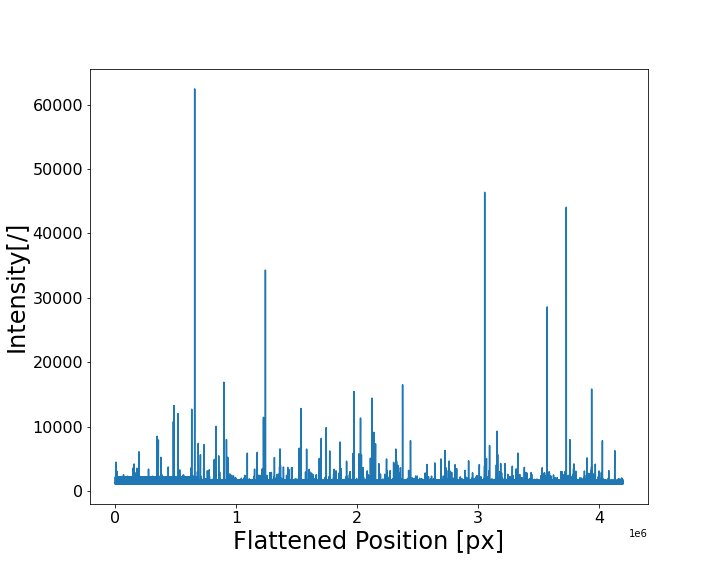
\includegraphics[width=7cm]{darkflame_average_ravel.png}
    \label{fig:darkflame_average_ravel}
}
\subfloat[ダークフレームのヒストグラム]{
    \centering
    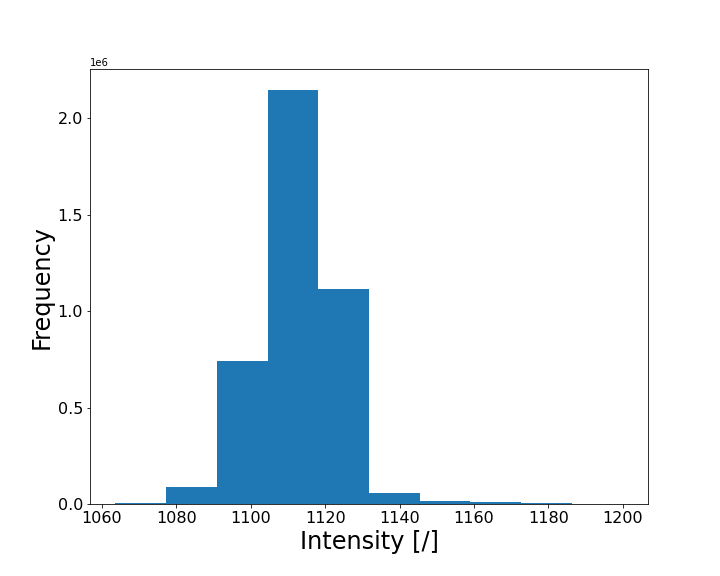
\includegraphics[width=7cm]{darkflame_average_histogram.png}
    \label{fig:darkflame_average_histogram}
}

\caption[]{平均ダークフレームにおける統計情報}
\label{fig:darkflame_average_stat}
\end{figure}

続いて、ダークフレームの撮影ごとの変化について目を向け、各ピクセルごとに求められるダークフレームに関しての統計情報を示す。

\begin{table}[!ht]
\begin{center}
  \begin{tabular}{|c|c|} \hline
    パラメータ & 値 \\ \hline
    最大値 & 3040.99 \\
    最小値 & 4.10 \\
    平均値 & 15.46 \\
    中央値 & 15.33 \\
    標準偏差 & 4.11 \\ \hline
  \end{tabular}
  \caption{ダークフレームの標準偏差の統計情報}
  \label{tb:darkflame_deviation_data}
\end{center}
\end{table}

\begin{figure}[!ht]
\centering

\subfloat[1次元化したダークフレーム標準偏差の強度分布]{
    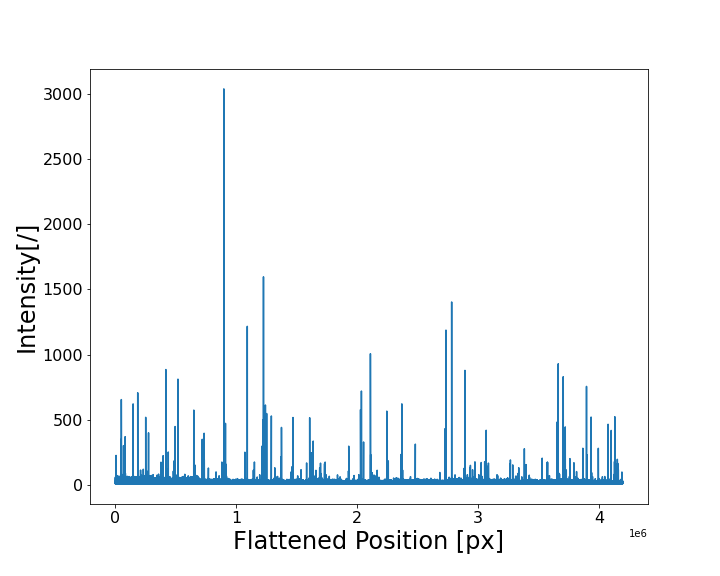
\includegraphics[width=7cm]{darkflame_deviation_ravel.png}
    \label{fig:darkflame_deviation_ravel}
}
\subfloat[ダークフレーム標準偏差のヒストグラム]{
    \centering
    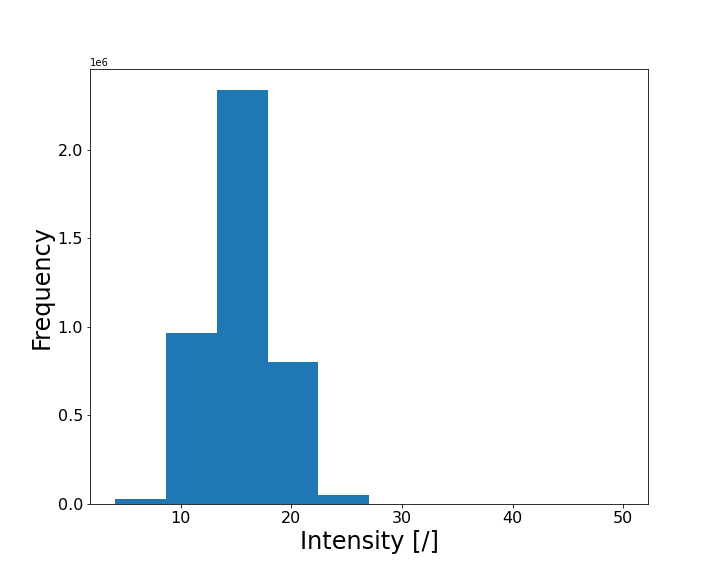
\includegraphics[width=7cm]{darkflame_deviation_histogram.png}
    \label{fig:darkflame_deviation_histogram}
}

\caption[]{ダークフレーム標準偏差における統計情報}
\label{fig:darkflame_deviation_stat}
\end{figure}

平均ダークフレームに関して、全体として1000程度のオフセットがあり、これは実験室内の機器の光が漏れてCCDカメラに入射しているものと考えられる。
またごく少数(20ピクセル程度)ではあるが、10000を超えるような値を取っているピクセルがあり、そのようなピクセルの標準偏差はいずれも1\%以下程度であるためこれは素子が不能になっているものと考えられる。
また15枚のダークフレーム間での標準偏差に関して、この平均値は十分に小さく撮影ごとの変化は大きくないと言える。

\subsection{ダークフレームの除去}
\ref{chap5_darkflame_measurement}節の計測により、ダークフレームの撮影ごとの変化はかなり小さいこと、また実験室内に存在する外乱光の影響で全体に1000程度の強度が乗ることが分かった。
外乱光の除去のため、計測開始の直前に計8枚のダークフレームを取得し、単純加算平均の結果を計測データから差し引いた。

\clearpage

% ================================================== %
% section
% ================================================== %
\newpage

\section{下流端走査タイコグラフィの結果}
\label{chap5_mirror_transverse_result}

\subsection{回復結果}

\begin{figure}[!ht]
\centering
\subfloat[回復された位相分布]{
    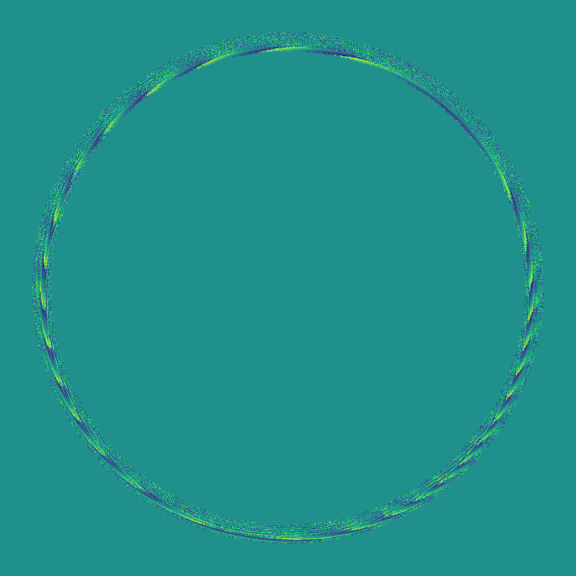
\includegraphics[width=7cm]{reconstructed_phase_before_unwrap.png}
    \label{fig:reconstructed_phase_before_unwrap}
}
\subfloat[位相アンラップ後の位相分布]{
    \centering
    
\includegraphics[width=7cm]{reconstructed_phase_unwrapped.png}
    \label{fig:reconstructed_phase_unwrapped}
}
\caption[]{回復された位相分布の位相アンラップ}
\label{fig:reconstructed_phase_unwrapping}
\end{figure}


\begin{figure}[!ht]
\centering
\subfloat[回復された位相分布(極座標)]{
    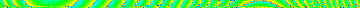
\includegraphics[width=7cm]{reconstructed_phase_before_unwrap_polar.png}
    \label{fig:reconstructed_phase_before_unwrap_polar}
}
\subfloat[位相アンラップ後の位相分布(極座標)]{
    \centering
    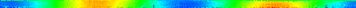
\includegraphics[width=7cm]{reconstructed_phase_unwrapped_polar.png}
    \label{fig:reconstructed_phase_unwrapped_polar}
}
\caption[]{回復された位相分布の位相アンラップ(極座標)}
\label{fig:reconstructed_phase_unwrapping_polar}
\end{figure}

輪帯幅のちょうど半分に当たる部分について回転角度方向にプロファイルを取ると、非点収差にあたる$\sin(\theta)$の成分が現れた。
これを$A \sin(\theta + \theta_0)$の形で最小自乗フィッテイングして重ねたものが図\ref{fig:astigmatism_fitted}である。
また、その差分を図\ref{fig:astigmatism_canceled}に示す。

ここで、真円度測定器RoncorderEC1550によって測定された周方向誤差プロファイルを図\ref{fig:roundness_error}に示す。
図\ref{fig:roundness_error_each}は上流側(放物面側)からの光軸方向距離$z$に応じてその周方向誤差を計測したプロファイルであり、図\ref{fig:roundness_error_average}はその単純平均である。

\begin{figure}[!ht]
\centering
\subfloat[光軸方向の各位置での周方向誤差プロファイル]{
    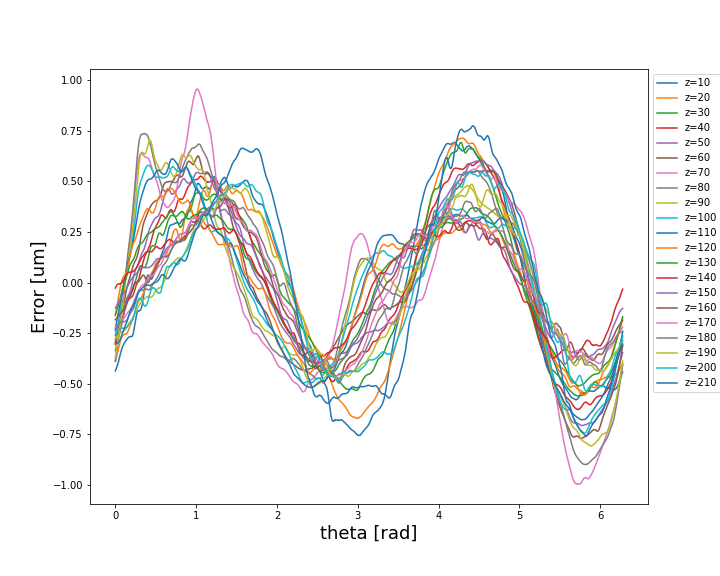
\includegraphics[width=7cm]{roundness_error_each.png}
    \label{fig:roundness_error_each}
}
\subfloat[平均化された周方向誤差プロファイル]{
    \centering
    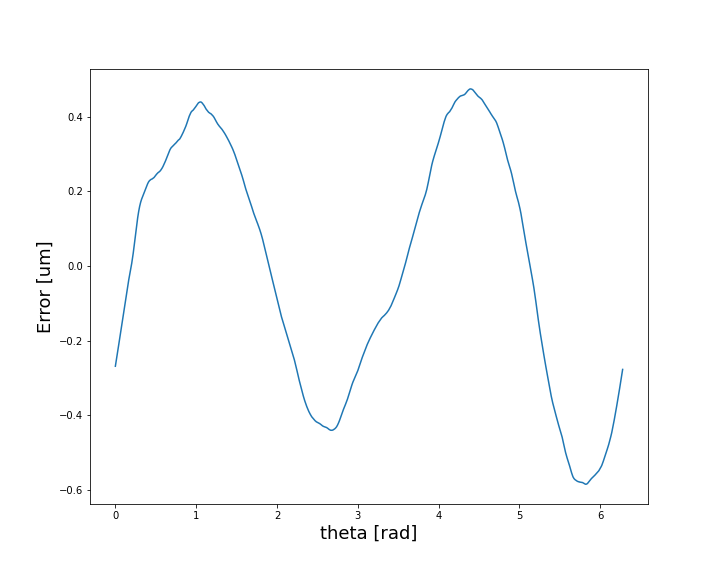
\includegraphics[width=7cm]{roundness_error_average.png}
    \label{fig:roundness_error_average}
}
\caption[]{真円度測定器での周方向誤差プロファイル測定結果}
\label{fig:roundness_error}
\end{figure}

回復された位相の周方向分布においてフィッティングされた非点収差成分は、その振幅が7.68 rad ($1.22\lambda$)であった。
これを周方向誤差量に換算すると\SI{101.5}{\micro \metre}程度になり、これがミラーによるものであるとすると真円度測定結果と大きく矛盾するため、非点収差がミラーに起因するものであるかどうかを確認する。
焦点面における強度分布を撮影すると、図\ref{fig:astigmatism_focus_before_rotation}のようであり、確かに集光点が円形ではなく十字の広がりを持っており、非点収差が存在することが確認できる。
続いて、ミラーを45度程度回転し、同様に焦点面における強度分布を撮影したものが図\ref{fig:astigmatism_focus_after_rotation}である。
ミラーに起因する非点収差であればミラーの回転に伴って集光点のパターンが回転するはずだが、ほとんど変わらない分布を示している。
これにより、位相回復結果から算出された非点収差はミラーより上流側の入射ビームの生成において生じたものであると結論付けることができる。


\begin{figure}[!ht]
\centering
\subfloat[輪帯中央における位相分布とsinフィッティング]{
    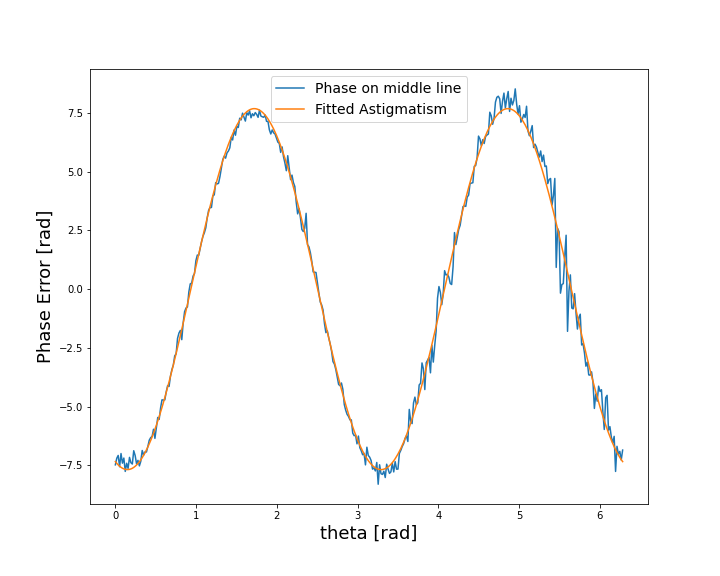
\includegraphics[width=7cm]{astigmatism_fitted.png}
    \label{fig:astigmatism_fitted}
}
\subfloat[非点収差成分を差し引いた位相分布]{
    \centering
    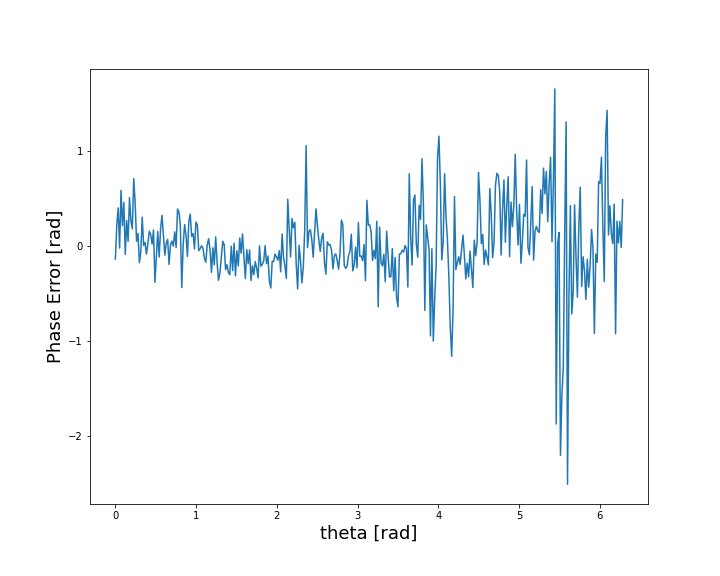
\includegraphics[width=7cm]{astigmatism_canceled.png}
    \label{fig:astigmatism_canceled}
}
\caption[]{回復された位相分布の位相アンラップ(極座標)}
\label{fig:astigmatism_analysis}
\end{figure}


\begin{figure}[!ht]
\centering
\subfloat[回転前の焦点面強度分布]{
    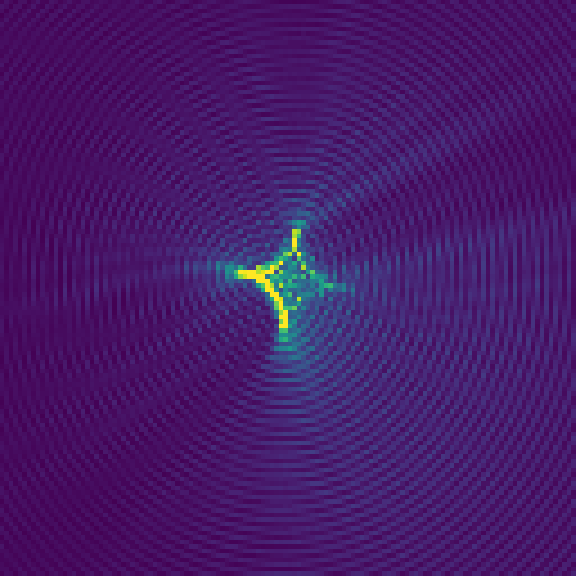
\includegraphics[width=7cm]{before_rotation.png}
    \label{fig:astigmatism_focus_before_rotation}
}
\subfloat[回転後の焦点面強度分布]{
    \centering
    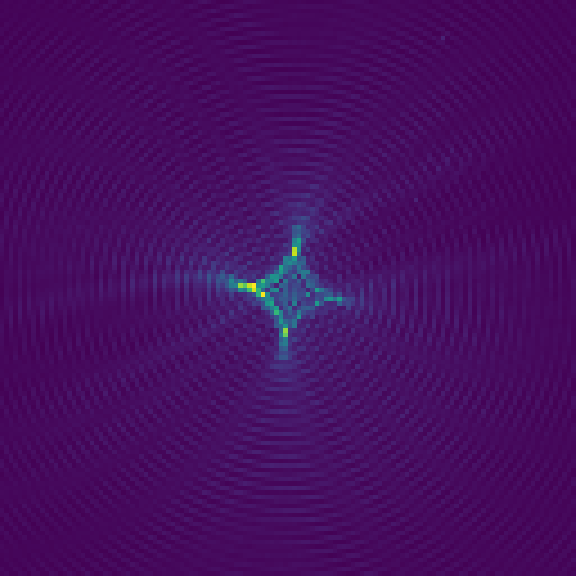
\includegraphics[width=7cm]{after_rotation.png}
    \label{fig:astigmatism_focus_after_rotation}
}
\caption[]{回転前後の焦点面強度分布}
\label{fig:darkflame_deviation_stat}
\end{figure}

% ================================================== %
% section
% ================================================== %
\section{結論}
\label{chap5_conclusion}


%%%%%%%%%%%%%%%%%%%%%%%%%%%%%%%%%%%%%%%%%%%%%%%%%%%%%%%%%%%%%%%%%%%%%%%%%%%%%

%%% Local Variables:
%%% mode: katex
%%% TeX-master: "../thesis"
%%% End:
